% a simple template with cesbio color code

\documentclass[xcolor=table, t, aspectratio=169]{beamer} 
\graphicspath{{../FIGURES/}}
\usepackage[utf8]{inputenc}
\usepackage{booktabs, comment} 
\usepackage[absolute, overlay]{textpos} 
\usepackage{pgfpages}
\usepackage{caption}
\usepackage[font=footnotesize]{caption}
\usepackage{multirow}
\usepackage{hyperref}
\usepackage{blindtext}
\usepackage{amsmath}
\usepackage[makeroom]{cancel}
\usepackage{textpos}
\usepackage{tikz}
\usepackage{csquotes}
\usepackage{graphicx}


% CESBIO ADAPTED COLOURS 
\definecolor{colorLAERO}{RGB}{67, 141, 204}
\definecolor{forestgreen}{rgb}{0.13, 0.55, 0.13}
\definecolor{greenyellow}{rgb}{0.68, 1.0, 0.18}
\definecolor{inchworm}{rgb}{0.7, 0.93, 0.36}

% OPTIONAL COLOURS
% you can add the ones you need : lot of proposition on http://latexcolor.com/
\definecolor{ballblue}{rgb}{0.13, 0.67, 0.8}
\definecolor{bluegreen}{rgb}{0.0, 0.87, 0.87}
\definecolor{chromeyellow}{rgb}{1.0, 0.65, 0.0}
\definecolor{darkcyan}{rgb}{0.0, 0.55, 0.55}
\definecolor{darkpastelred}{rgb}{0.76, 0.23, 0.13}
\definecolor{electricgreen}{rgb}{0.0, 1.0, 0.0}
\definecolor{electriclime}{rgb}{0.8, 1.0, 0.0}
\definecolor{deepcarrotorange}{rgb}{0.91, 0.41, 0.17}
\definecolor{ganttblue}   {HTML}{2B6CB0}
\definecolor{ganttcyan}   {HTML}{2C7A7B}
\definecolor{ganttgreen}  {HTML}{276749}
\definecolor{ganttorange} {HTML}{C05621}
\definecolor{ganttgray}   {HTML}{4A5568}
\definecolor{ganttbg}     {HTML}{EBF4FF}
\definecolor{ganttbar}    {HTML}{BEE3F8}
\definecolor{milestonecol}{HTML}{E53E3E}


% CESBIO ADAPTED BEAMER OPTIONS
\setbeamercolor{title in head/foot}{bg=inchworm, fg=forestgreen}
\setbeamercolor{author in head/foot}{bg=colorLAERO}
\setbeamertemplate{page number in head/foot}{}

\useoutertheme{infolines}
\usetheme{Warsaw}
\usecolortheme[named=colorLAERO]{structure}


% SPECIFIC COMMANDS
% if you nee to set command for youe presentation, you can put them here
\newcommand{\defnotation}[1]{\bf{\textsl{#1}}}

\usepackage[
citestyle=abbrv, 
bibstyle=abbrv,
style=authoryear, %-comp,
backend=biber
%maxbibnames=99, % Make sure we are printing all authors in the appendix
]{biblatex}

\usepackage{pgfgantt}
\usepackage{helvet}
% PRESENTATION INFORMATIONS
% to fill in

% \title[]{}
% \subtitle{Subtitle}

\usetikzlibrary{positioning, calc}
\usetikzlibrary{calc}

% ── Colours (adapt to your theme) ─────────────────────────────────────────────
\definecolor{titleblue}  {HTML}{1A365D}
\definecolor{accentblue} {HTML}{2B6CB0}
\definecolor{lightgray}  {HTML}{EDF2F7}
\definecolor{medgray}    {HTML}{718096}

% ── Metadata ──────────────────────────────────────────────────────────────────
\author[J.~Hedman]{Johan Hedman}
\institute[LAERO]{Laboratoire d'Aérologie (LAERO) · Université de Toulouse}
\date{\today}

% ── Title frame ───────────────────────────────────────────────────────────────
% Use a fully custom frame instead of \titlepage for full layout control
\newcommand{\customtitleframe}{%
\begin{frame}[plain]
	\begin{tikzpicture}[remember picture, overlay]
		
		%% ── Background ─────────────────────────────────────────────────────────────
		\fill[titleblue]
		(current page.north west) rectangle
		($(current page.north east) + (0, -0.38\paperheight)$);
		
		\fill[accentblue]
		($(current page.north west) + (0, -0.38\paperheight)$) rectangle
		($(current page.north east) + (0, -0.405\paperheight)$);
		
		%% ── Title block ────────────────────────────────────────────────────────────
		\node[anchor=west, text=white, font=\large\bfseries, text width=0.95\paperwidth,] at 
		($(current page.north west) + (0.7cm, -0.13\paperheight)$)
		{Etude des rouleaux de couche limite sous les tempêtes};
		
		\node[anchor=west, text=white!70!titleblue, font=\small,text width=0.85\paperwidth,] at 
		($(current page.north west) + (0.7cm, -0.26\paperheight)$)
		{Johan Hedman \quad·\quad LAERO, Université de Toulouse \quad·\quad \insertdate};
		
		%% ── Supervisors ────────────────────────────────────────────────────────────
		\node[anchor=north west, font=\bfseries\small\color{accentblue}] at 
		($(current page.north west) + (0.7cm, -0.405\paperheight - 0.52cm)$)
		{Supervision};
		
		\node[anchor=north west, font=\footnotesize\color{titleblue}, align=left, text width=0.38\paperwidth]
		at ($(current page.north west) + (0.7cm, -0.405\paperheight - 1.0cm)$)
		{%
			\textbf{Prof. Jean-Pierre Chaboureau} \\
			\textcolor{medgray}{LAERO, Université de Toulouse} \\[5pt]
		};
		
		%% ── Divider ────────────────────────────────────────────────────────────────
		\draw[accentblue!30, line width=0.5pt]
		($(current page.north west) + (0.50\paperwidth, -0.405\paperheight - 0.50cm)$) --
		($(current page.south west) + (0.50\paperwidth, 0.45cm)$);
		
		%% ── Jury ───────────────────────────────────────────────────────────────────
		\node[anchor=north west, font=\bfseries\small\color{accentblue}]at ($(current page.north west) + (0.53\paperwidth, -0.405\paperheight - 0.52cm)$)
		{Membre du CSI};
		
		\node[anchor=north west, font=\footnotesize\color{titleblue}, align=left, text width=0.42\paperwidth]
		at ($(current page.north west) + (0.53\paperwidth, -0.405\paperheight - 1.0cm)$)
		{%
			\textbf{Prof } \textcolor{medgray}{\textit{}} \\
			\textbf{Prof.~Firstname Lastname} \textcolor{medgray}{\textit{}} \\
		};
		
		%% ── Logo strip ─────────────────────────────────────────────────────────────
		\fill[white]
		($(current page.south west) + (0, 0.10\paperheight)$)
		rectangle (current page.south east);
		
		\draw[accentblue!25, line width=0.4pt]
		($(current page.south west) + (0, 0.10\paperheight)$) --
		($(current page.south east) + (0, 0.10\paperheight)$);
		
		\node[anchor=south west, xshift=0.5cm, yshift=0.20cm] at (current page.south west)		{
\includegraphics[height=1.5cm]{LOGO/LAERO-logo.jpg}};
		
		\node[anchor=south, yshift=0.25cm] at (current page.south)
			{
\includegraphics[height=1.0cm]{LOGO/UNIV-logo.png}\hspace{1cm}%
			
\includegraphics[height=1.20cm]{LOGO/CNRS-logo.jpeg}};
		
		\node[anchor=south east, xshift=-0.5cm, yshift=0.20cm] at (current page.south east)
		{
\includegraphics[height=1.2cm]{LOGO/logo-IRD.png}};
		
	\end{tikzpicture}
\end{frame}
}





% cesbio adapted frame structure
\addtobeamertemplate{navigation symbols}{}{%
    \usebeamerfont{footline}%
    \usebeamercolor[fg]{footline}%
    \hspace{1em}%
    \insertframenumber/\inserttotalframenumber
}

\usepackage{soul}
\makeatletter
\let\HL\hl
\renewcommand\hl{%
  \let\set@color\beamerorig@set@color
  \let\reset@color\beamerorig@reset@color
  \HL}
\makeatother

\addbibresource{../../groupeThese.bib}
\graphicspath{{FIGURES/}}

\AtBeginSection[]{%
	\begin{frame}[plain]
		\vfill
		\begin{tikzpicture}[remember picture, overlay]
			% Background color block on the left
			\fill[titleblue] (current page.north west) rectangle 
			([xshift=0.4\paperwidth]current page.south west);
		\end{tikzpicture}
		
		% Left side: big section number + title
		\begin{columns}[c]
			\begin{column}{0.38\textwidth}
				\begin{flushright}
					{\color{white}\fontsize{60}{60}\selectfont
						\thesection}\\[0.3em]
					{\color{white}\Large\bfseries
						\insertsectionhead}
				\end{flushright}
			\end{column}
			
			\hspace{0.04\textwidth}
			
			% Right side: subsection list
			\begin{column}{0.52\textwidth}
				\tableofcontents[
				currentsection,
				sectionstyle=hide,
				subsectionstyle=show/show/hide,
				]
			\end{column}
		\end{columns}
		\vfill
	\end{frame}
}

\usepackage[caption = false]{subfig}
\begin{document}
	

%\customtitleframe
	
%% ============================================================================
% =============================================================================
% =============================================================================
\section{Introduction au sujet}
%% ============================================================================
% =============================================================================
% =============================================================================

\subsection{Qu'est ce que les rouleaux de couche limite ?}
\begin{frame}{Qu'est ce que les rouleaux de couche limite ?}
			\vfill
	\begin{minipage}{0.35\textwidth}
	\centering
		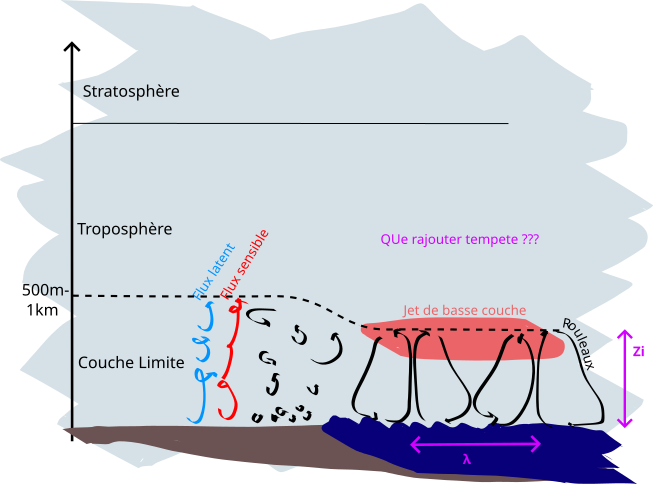
\includegraphics[width=\linewidth]{INTRO/intro.png}
	\end{minipage}
	\hfill
	\begin{minipage}{0.55\textwidth} 
	Autres noms: circulations secondaire, structures, ... => Structure cohérentes de turbulence. \\
	Caractéristiques principales (\cite{etlingRollVorticesPlanetary1993}): 
		\begin{itemize}
			\item De la hauteur de la Couche Limite $z_i$.
			\item 2-5 fois la largeur de la Couche Limite : $\lambda / z_i = 2-5 $ 
			\item angle de -+ 10/30 deg aligné avec la direction du vent (cf Ekmann ??) 			
		\end{itemize}
	\end{minipage}
	\vfill
\end{frame}

\subsection{Pourquoi s'y intéresser ?}
\begin{frame}{Pourquoi s'y intéresser ?}
	
	organisation de la turbulence : impact sur les flux 
	convection peu profonde 
	modifie l'écoulemnt : impt en cas de vent fort
	
	cf ligne de grain
	
	\cite{lfarhDownwardTransportStrong2023}
	\cite{riviereDownwardTransportMomentum2020}
	
	
	Transport de quantité de mouvement vers la surface
	échange avec la surface
	différent des thermiques 
	structure organisée

\end{frame}

\subsection{Où sont-ils observés ?}
\begin{frame}{Où sont-ils observés ?}
	Observation via satellite dans le visible (rue de nuage) ou radar SAR (rugosité de la mer) ou observation au sol (Lidar, radar)
	
	\vfill
	\begin{minipage}{0.65\textwidth}
		Graphe résume certaine obs et ref de rolls \\
		Brümmer et al CAO \\
		Foster 2005: \\
	\end{minipage}
	\hfill
	\begin{minipage}{0.3\textwidth} 
		\begin{figure}
			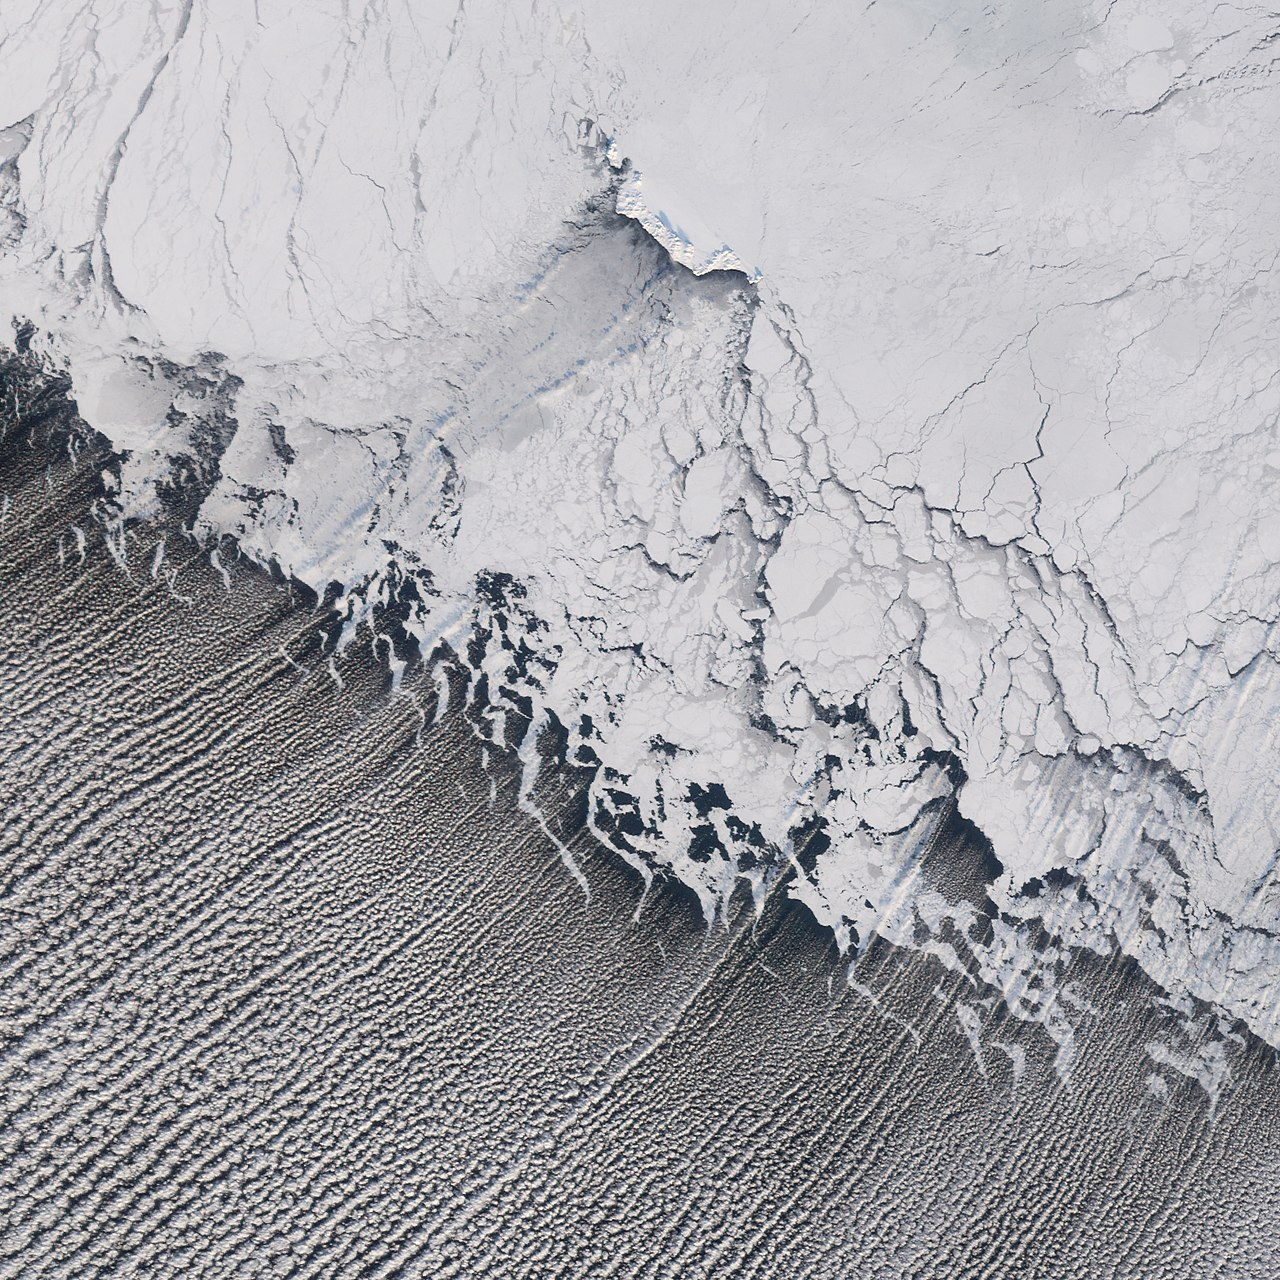
\includegraphics[width=0.8\textwidth]{roll.jpg}
			\caption{Rouleaux durant épisode de froid au-dessus de la mer de Barents (NOAA 7, AVHRR,6.4.1988)}
		\end{figure}
	\end{minipage}
	\vfill

	
\end{frame}

\subsection{Comment se forment-ils ?}
\begin{frame}{Comment se forment-ils ?}
Différentes instabilités (\cite{etlingRollVorticesPlanetary1993}):
\begin{itemize}
\item Instabilité point d'inflection (théorème de Rayleigh, Brown 1980)
\item Instabilité parallèles, pour un fluide en rotation 
\item \textbf{Instabilité thermique} (Rayleigh Bénard) 
\end{itemize}

\vfill

	Ref sur leur étude 
	écoulemetn Rayleigh Benard Couette 
	ex Gryscka 
	ex Foster 
\end{frame}

\subsection{Quelles sont mes questions scientifiques ?}
\begin{frame}{Quelles sont mes questions scientifiques ?}

\end{frame}



%% =======================================================================
% ========================================================================
% ========================================================================
\section{1re partie de la thèse}
%% =======================================================================
% ========================================================================
% ========================================================================

\subsection{Point de départ des simulations}
\begin{frame}{Tempête ALEX (et Adrian?)}
Pk interet ? 
présentation des tempêtes 
présence de rouleaux, obs ? 
\end{frame}

\subsection{Couche limite de tempête idéalisée}
\begin{frame}{Simulations idéalisées}
Quel est le but ? 
les enjeux ? 
objectfof ? 
point de départ ? 
\end{frame}

\subsection{Justification de la méthode}
\begin{frame}{Justification de la méthode}
	NAWDIC blabla
\end{frame}

\subsection{Comparaison cas réel - cas idéalisé}
\begin{frame}{Comparaison cas réel - cas idéalisé}
	NAWDIC blabla
\end{frame}

\subsection{Etude sensi ??}
\begin{frame}{Etude sensi ??}
	NAWDIC blabla
\end{frame}


%% =======================================================================
% ========================================================================
% ========================================================================
\section{2e partie de la thèse}
%% =======================================================================
% ========================================================================
% ========================================================================

\subsection{Presentation vol NAWDIC}
\begin{frame}{Etude sensi ??}
	NAWDIC blabla
\end{frame}


\subsection{Pourquoi ce vol ? }
\begin{frame}{Etude sensi ??}
	NAWDIC blabla
\end{frame}


\begin{frame}{Analyse risque}
	\vfill
	\begin{itemize}
		\item \textbf{Force} : Beaucoup de travail mis sur LES idéalisée, bonne connaissance mesoNH (moi et entourage)
		\item \textbf{Faiblesse} : Pas de formation de base en atmosphère (possibilité de manquer des idées); 
								pas de spécialité en CLA dans l'encadrement
		\item \textbf{Opportunités} : Campagne NAWDIC (mesures et possibilités de collaboration)
		\item \textbf{Menaces} : IA ? Comment s'insérer dans ce contexte ? 
	\end{itemize}
\end{frame}


\section{Formations}
\begin{frame}{Formations}
	contenu...
\end{frame}

\begin{frame}{Conclusion}
	\printbibliography
\end{frame}

\end{document}   
